      \begin{figure*}[hbt]
        \begin{minipage}{0.46\linewidth}
          \begin{center}
            % 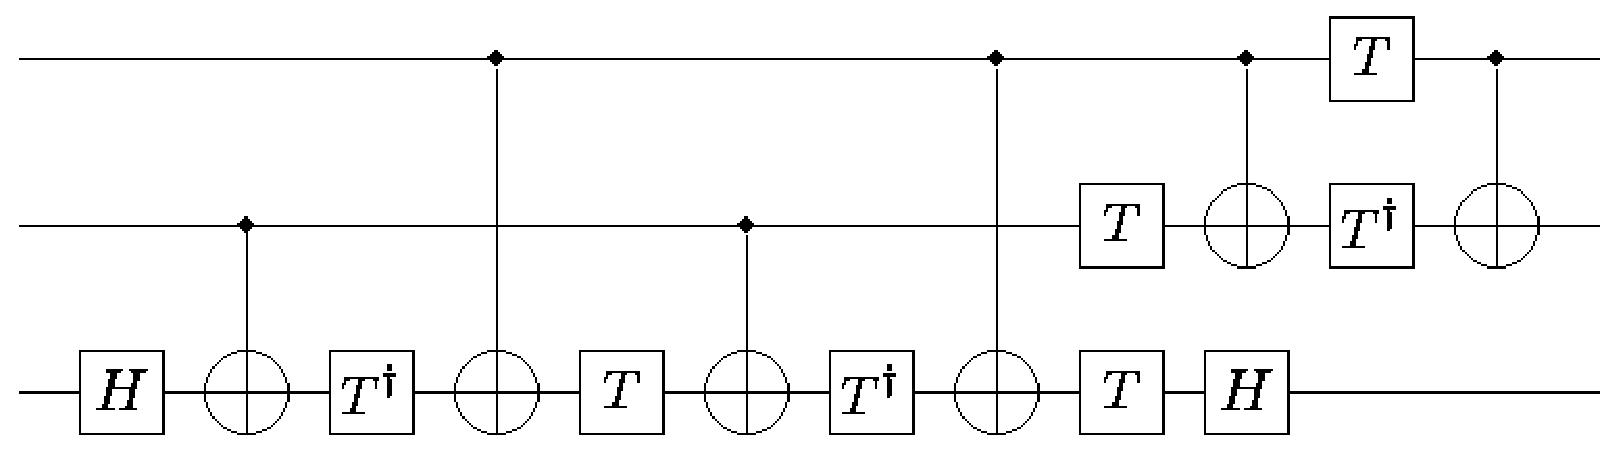
\includegraphics[width=6cm]{img/toffoli.eps}
           % 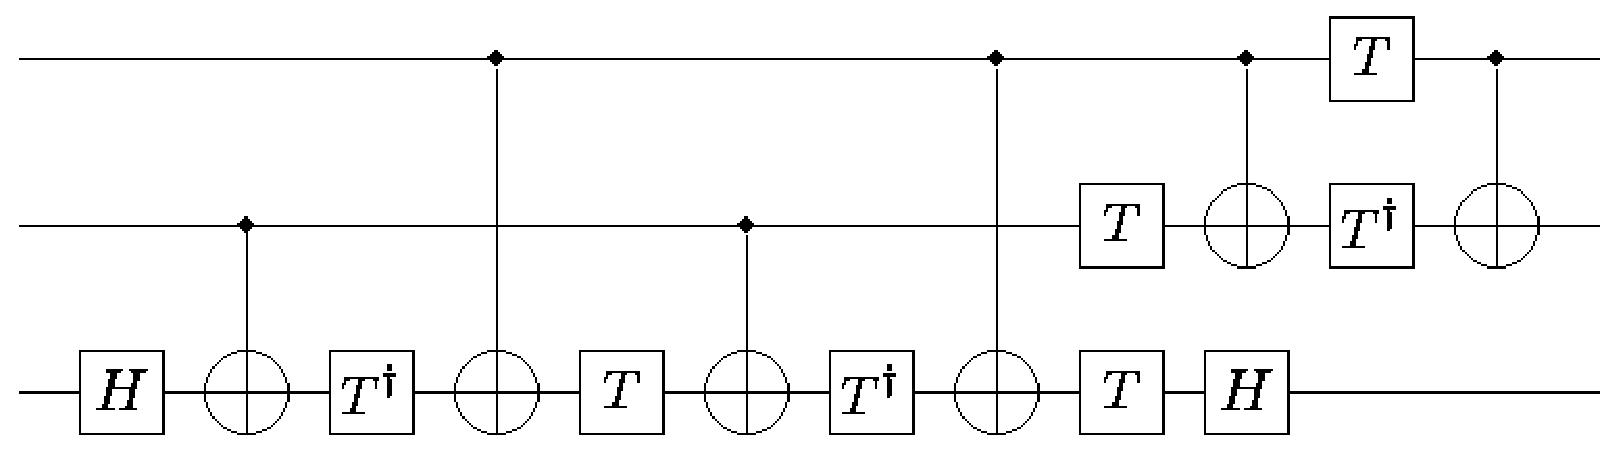
\includegraphics[width=\linewidth]{img/toffoli.eps}
            \Qcircuit @C=0.5em @R=0.2em @!R { \\
          \lstick{{x}_{0}} & \ctrl{2} & \qw &    & & \push{{x}_{0} :  } & \qw & \qw & \qw & \ctrl{2} & \qw & \qw & \qw & \ctrl{2} & \ctrl{1} & \gate{\mathrm{T}} & \ctrl{1} & \qw & \qw\\
          \lstick{{x}_{1}} & \ctrl{1} & \qw & \push{=}   & &\push{{x}_{1} :  } & \qw & \ctrl{1} & \qw & \qw & \qw & \ctrl{1} & \gate{\mathrm{T}} & \qw & \targ & \gate{\mathrm{T^\dagger}} & \targ & \qw & \qw\\
          \lstick{{f}}    & \targ \qw   & \qw &    & &  \push{{f} :  } & \gate{\mathrm{H}} & \targ & \gate{\mathrm{T^\dagger}} & \targ & \gate{\mathrm{T}} & \targ & \gate{\mathrm{T^\dagger}} & \targ & \gate{\mathrm{T}} & \gate{\mathrm{H}} & \qw & \qw & \qw\\
}

            \caption{A Toffoli gate in Clifford+T basis}
            \label{fig-toffoli}
          \end{center}
        \end{minipage}
        \hspace*{10mm}
        \begin{minipage}{0.46\linewidth}
          \begin{center}
            % \includegraphics[width=6cm]{img/rtof.eps}
            %\includegraphics[width=\linewidth]{img/rtof.eps}
            \Qcircuit @C=0.5em @R=0.2em @!R { \\
          \lstick{{x}_{0}} & \ctrl{2}\qw          & \qw &          & & \qw               & \qw               & \qw      & \qw                       & \ctrl{2} & \qw               & \qw      & \qw                         & \qw                &\qw\\
          \lstick{{x}_{1}} & \ctrl{1}             & \qw & \push{=} & & \qw               & \qw               & \ctrl{1} & \qw                       & \qw      & \qw               & \ctrl{1} & \qw                         & \qw                &\qw\\
          \lstick{{x}_{3}} & \push{\rtoftarg}\qw  & \qw &          & & \gate{\mathrm{H}} & \gate{\mathrm{T}} & \targ    & \gate{\mathrm{T^\dagger}} & \targ    & \gate{\mathrm{T}} & \targ    & \gate{\mathrm{T^{\dagger}}} & \gate{\mathrm{H}}  &\qw
}

            \caption{An RTOF gate in Clifford+T basis}
            \label{fig-rtof}
          \end{center}
        \end{minipage}
      \end{figure*}

    % ToffoliゲートとRTOFゲートの違いは，
    % RTOFゲートは入力によって回路の位相を変化させる場合があることにある．
    % 図\ref{rtof}に示すRTOFの全ての入力に対する位相は，表\ref{table-rtof}に示す通りである．
    % RTOFゲートの入力（$x_1, x_2, x_3$）が
    % $(1, 1, 0),(1, 0, 1), (1, 1, 1)$のとき，位相はそれぞれ，
      % $+\frac{\pi}{2}, +\pi, -\frac{\pi}{2}$だけ変化する．
\begin{figure*}[ht]
  \def\@captype{table}
  \begin{minipage}[ht]{.46\textwidth}
    \begin{center}
       %\scalebox{0.7}[1]{
        \begin{tabular}{c|c}      \hline
          input & $\Delta\theta$  \\\hline
          000   & 0      \\
          001   & 0      \\
          010   & 0      \\
          011   & 0      \\
          100   & 0      \\
          101   & $+\pi$          \\
          110   & $+\pi/2$   \\
          111   & $-\pi/2$ \\ \hline
        \end{tabular}        
    \end{center}
        \captionof{table}{Added phases by an RTOF.}
        \label{table-rtof}
  \end{minipage}
  \begin{minipage}[ht]{.46\textwidth}
    \begin{center}
      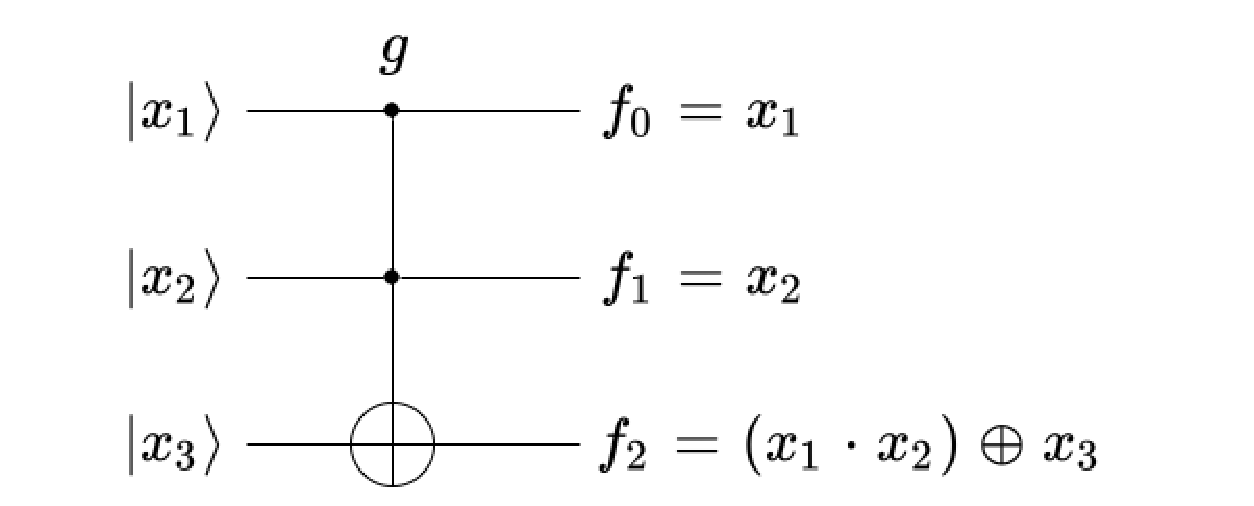
\includegraphics[width=5cm]{img/toffoli-f.eps}
      \caption{Functional representations for the output of a Toffoli gate.}
      \label{toffoli-f}
    \end{center}
  \end{minipage}

  
  %
 \end{figure*}

\section{Introduction}

Boolean functions are often used as essential components in quantum algorithms, such as oracles and cost functions; these are often calculated using the circuit model called {\it quantum Boolean circuits}~\cite{bib-circuit}. To realize such quantum Boolean circuits, a Toffoli gate is often used as a logic primitive. However, as three qubit operations do not occur naturally in the two level systems that modern quantum computers are made of, these Toffoli gates have to be in turn, composed of physically realizable gates, such as NOT, CNOT, and T. (e.g., the Clifford+T~\cite{bib-gates} basis gate set), as depicted in Fig.~\ref{toffoli}

As qubits are famously prone to error and perturbation, it is often useful to consider a {\it fault-tolerant} implementation of quantum computation, one which could detect and correct errors ~\cite{bib-mike-and-ike}. Unfortunately, in the fault-tolerant paradigm, T-gates incur much higher cost than so-called Clifford gate types. Many of the most prominent implementations employ state purification and gate teleportation, among others. Because of its relatively outsized cost compared to Clifford gates, it has the possibility of overwhelming the base cost of a particular circuit implementation. As T gates are key to quantum advantage, due to the Gottesman-Knill Theorem, decreasing the number of T-gates (T-count) has been identified as of paramount importance in bridging the gap between theoretical models of quantum computation and their physically realizable counterparts, and many propositions have been made to decrease their number in a given circuit.

Our research seeks to leverage recent results in relative phase implementations of Boolean functions ~\cite{bib-rtof-maslov} ~\cite{bib-amy-phase-state} and LUT-based quantum circuit synthesis to reduce T-count in a a qubit constrained environment.

\noindent {\bf Our Contribution.} 
We propose a method that reduces the number of T-gates in a Quantum LUT Network by exploiting relative phase Boolean functions. Among our contributions:
\begin{itemize}
\item A novel method to synthesize a Boolean function up to a relative phase by utilizing relative phase constructions and Shannon Decomposition
\item A method to generate a Quantum Boolean Circuit from a Boolean Logic Network representation leveraging the above method to reduce T-count

\end{itemize}
Our methods are compared to a naive synthesis of each LUT node that utilizes an ESOP-based method to synthesize each Boolean function exactly as a Quantum Boolean Circuit. We find that on average, for similar usage of ancilla qubits, this improves T-count by DCTODO\%. While there remain a few exceptions to its advantage, its advantage in the majority of cases we have tested points to more resea

The paper is structured as follows. Section~\ref{Sec:prelim} outlines preliminary information for understanding this paper. Then Section~\ref{Sec:Exist} lays out some motivations for the research we are going to conduct. Section~\ref{Sec:proposed} follows with our proposed method, including our novel method to realize functions up to a relative phase without any additional ancillae, and then its use with the LHRS. Then, Our experimental results in Section~\ref{Sec:exp} can confirm that our method can indeed reduce the T-count of quantum Boolean circuits. Finally Section~\ref{Sec:concl} concludes the paper with our conclusions and future work.

